\documentclass[11pt]{article}

\usepackage[margin=0.88in,headheight=15pt]{geometry}
\usepackage[T1]{fontenc}
\usepackage{lmodern}
\usepackage{microtype}
\usepackage{amsmath,amssymb,mathtools}
\usepackage{booktabs,longtable,tabularx,array}
\usepackage{graphicx}
\usepackage[dvipsnames,table]{xcolor}
\usepackage{enumitem}
\usepackage{fancyhdr}
\usepackage[hidelinks]{hyperref}
\usepackage[nameinlink,noabbrev]{cleveref}

\definecolor{ink}{HTML}{17212B}
\definecolor{blue}{HTML}{176B87}
\definecolor{paleBlue}{HTML}{EAF4F7}
\definecolor{green}{HTML}{277A53}
\definecolor{orange}{HTML}{A85D00}
\definecolor{red}{HTML}{A33333}
\definecolor{gray}{HTML}{5A6570}

\hypersetup{
  colorlinks=true,
  linkcolor=blue,
  urlcolor=blue,
  citecolor=blue,
  pdftitle={Harmonic-coordinate worldtube matching},
  pdfsubject={Analytic structure and numerical findings from q=4 and q=8 virtual worldtubes}
}

\pagestyle{fancy}
\fancyhf{}
\fancyhead[L]{\small\color{gray}Harmonic-coordinate worldtube matching}
\fancyhead[R]{\small\color{gray}Working report}
\fancyfoot[C]{\thepage}
\renewcommand{\headrulewidth}{0.4pt}
\renewcommand{\footrulewidth}{0pt}

\setlist[itemize]{leftmargin=1.5em,itemsep=0.25em,topsep=0.4em}
\setlist[enumerate]{leftmargin=1.7em,itemsep=0.3em,topsep=0.4em}
\setlength{\parindent}{0pt}
\setlength{\parskip}{0.48em}
\setlength{\tabcolsep}{5pt}
\renewcommand{\arraystretch}{1.12}

\newcommand{\eps}{\epsilon}
\newcommand{\G}{G}
\newcommand{\Rop}{\mathcal R}
\newcommand{\E}{\mathcal E}
\newcommand{\B}{\mathcal B}
\newcommand{\Kretsch}{\mathcal K}
\newcommand{\status}[2]{\textcolor{#1}{\textbf{#2}}}
\newcommand{\alg}{\status{green}{algebraically verified}}
\newcommand{\num}{\status{blue}{numerically verified}}
\newcommand{\prov}{\status{orange}{provisional}}
\newcommand{\openstatus}{\status{red}{open}}

\graphicspath{{q8_harmonic_worldtube_report_figures/}{figures/}}

\title{\vspace{-1.4cm}
  \textbf{\color{ink}Harmonic-coordinate worldtube matching}\\[0.35em]
  \large Analytic structure and numerical findings from\\
  \(q=4\) and \(q=8\) virtual worldtubes}
\author{}
\date{29 July 2026}

\begin{document}
\maketitle
\vspace{-1.2em}

\begin{center}
\begin{minipage}{0.92\textwidth}
\colorbox{paleBlue}{%
\parbox{\dimexpr\linewidth-2\fboxsep\relax}{%
\textbf{Purpose.}
This report is the interpretive companion to
\texttt{q8\_first\_order\_matching.ipynb}.  The notebook contains the
executable block solves, manufactured tests, closure diagnostics, radial
derivatives, random-point validation, second-order sensitivity analysis, and
Gauss--Seidel iteration.  The focused directory
\texttt{temporal\_ode\_consistency/} contains the multi-slice and direct
\(\Pi,\Phi\) time-derivative checks.
}}
\end{minipage}
\end{center}

\begin{abstract}
We investigate whether a tidally perturbed Schwarzschild metric in harmonic
coordinates can supply inner-boundary data from numerical binary-black-hole
simulations.  Expanding the coordinate map and inverse metric through second
order turns the matching problem into a hierarchy of linear overdetermined
systems once lower-order sources are fixed.  Component, parity, and STF
structure split those systems into small blocks whose coefficients can be
cross-checked in omitted multipoles, radial derivatives, and independent
interior points.

The first-order model gives a large and repeatable improvement over centered
Schwarzschild.  At \(q=8\), the provisional V1+C3 hierarchy reduces the
held-out inverse-metric RMS error from \(2.21\times10^{-1}\) to
\(3.61\times10^{-2}\).  Radial derivatives modestly improve the vector
sector.  The complete triangular 43-parameter second-order solve is
algebraically correct but fails cross-component and interior validation.
Sensitivity is concentrated in the symmetric spatial-strain rate and time
acceleration, while a targeted polar-\(J=2\) subsystem provides the strongest
larger second-order block.  Early-stopped block Gauss--Seidel iteration
reduces the interior error to approximately \(3.0\times10^{-2}\) on the
smallest worldtubes.

Direct metric time derivatives constructed from \(\Pi\), \(\Phi\), lapse,
and shift show that freely fitted second-order time jets were inflated by
roughly three orders of magnitude.  They also provide independent
measurements of first-order evolution and, through the fixed-inertial
translation response, a metric-only measurement of the center velocity.
\end{abstract}

\tableofcontents
\clearpage

\section{Scientific objective and scope}

The purpose of the worldtube construction is to replace the unresolved
interior of the smaller black hole by a local analytic metric whose
coefficients are measured from the numerical solution on a surrounding
sphere.  The local metric is a slowly evolving, tidally perturbed
Schwarzschild solution in harmonic coordinates.

The fit must accomplish more than interpolation on the fitting sphere.  A
useful matching model must:

\begin{enumerate}
  \item determine the coordinate transformation between the numerical
        inertial coordinates and local harmonic coordinates;
  \item measure the physical tidal fields and coordinate-map coefficients;
  \item predict metric component/STF blocks omitted from the solve;
  \item reproduce independent spatial and time derivatives;
  \item extrapolate the inverse metric to points inside the worldtube.
\end{enumerate}

Two simulations have been used:

\begin{itemize}
  \item a \(q=4\) calculation, principally at
        \(T=850M_{\rm tot}\), for the initial analytic and numerical audit;
  \item a more perturbative \(q=8\) calculation at
        \(T=950M_{\rm tot}\), together with ten slices through
        \(T=995M_{\rm tot}\), for the current block, derivative, and
        dynamical tests.
\end{itemize}

The black-hole mass \(M\) is fixed to its initial-data value.  It is not a
fitting parameter, and tidal heating enters beyond the retained order.  The
formal parameter \(\eps\) counts perturbative order.  It is set to one when a
complete truncated metric is evaluated; it is not a numerical velocity.

\subsection{Status vocabulary}

\begin{center}
\begin{tabularx}{0.92\textwidth}{>{\raggedright\arraybackslash}p{0.24\textwidth}X}
\toprule
\textbf{Status} & \textbf{Meaning}\\
\midrule
\alg & Independent symbolic constructions agree, or a manufactured identity
vanishes to roundoff.\\
\num & A stated claim has passed a simulation-data test with a recorded
diagnostic.\\
\prov & A trend is useful for designing the matching system but has not yet
been demonstrated across enough simulations, times, or resolutions.\\
\openstatus & The present analysis does not establish the claim.\\
\bottomrule
\end{tabularx}
\end{center}

\section{Coordinate map and perturbative organization}

Let \((t,\rho n^i)\) be local harmonic coordinates and \((T,X^i)\) the
simulation inertial coordinates.  At fixed harmonic slow time, the coordinate
map through second order is
\begin{align}
T={}&t+q^0
 +\eps\frac{\rho}{M}b_i n^i \notag\\
&+\eps^2\left[
  {\cal J}(\rho)\ddot q^0
 +{\cal K}(\rho)\dot b_i n^i
 +\Phi(\rho)Q_{ij}n^in^j
 -M(\rho^2-M^2)\E_{ij}n^in^j
\right]
+O(\eps^3),
\label{eq:time-map}\\
X^i={}&\rho n^i+q^i
 +\eps\frac{\rho}{M}L^i{}_j n^j \notag\\
&+\eps^2\left[
  {\cal J}(\rho)\ddot q^i
 +{\cal K}(\rho)\dot L^i{}_j n^j
 +\Phi(\rho)Q^i{}_{jk}n^jn^k
 +\text{electric-tidal radial profiles}
\right]
+O(\eps^3).
\label{eq:space-map}
\end{align}
Here
\begin{align}
{\cal J}(\rho)&=W_D(\rho)-\frac12\bigl(\rho_D^\star\bigr)^2,
&
{\cal K}(\rho)&=-2(\rho-2M),
&
\Phi(\rho)&=\frac12\left[3(\rho/M)^2-1\right],
\end{align}
with \(\rho_D^\star=r+2M\ln[r/(2M)]\) and \(r=\rho+M\).
The explicit electric profiles and the complete light-cone metric are
recorded in the analytic audit package; the present report concentrates on
how their response columns are used numerically.

\begin{center}
\small
\begin{tabularx}{0.96\textwidth}{
  >{\raggedright\arraybackslash}p{0.13\textwidth}
  >{\raggedright\arraybackslash}p{0.34\textwidth}
  >{\centering\arraybackslash}p{0.10\textwidth}X}
\toprule
\textbf{Order} & \textbf{quantity} & \textbf{count} & \textbf{role}\\
\midrule
\(\eps^0\) & \(q^i\), \(q^0\) & \(3+1\) &
spatial center and conventional time origin\\
\(\eps^1\) & \(\dot q^0\), \(b_i\), \(\dot q^i\), \(L_{(ij)}\) &
\(1+3+3+6\) & clock rate, time gradient, translational velocity, and
symmetric affine map\\
\(\eps^2\) & \(\ddot q^\mu\), \(\dot b_i\), \(\dot L_{(ij)}\) &
\(4+3+6\) & instantaneous time jets; evolution variables across slices\\
\(\eps^2\) & \(Q_{ij}\), \(Q^i{}_{jk}\) & \(5+15\) &
new harmonic-coordinate quadrupoles\\
\(\eps^2\) & \(\E_{ij}\), \(\B_{ij}\) & \(5+5\) &
physical electric and magnetic STF tensors\\
\bottomrule
\end{tabularx}
\end{center}

The local triad is taken to be nonrotating, so the antisymmetric part of
\(L^i{}_j\) is fixed by convention.  Inertial orbital motion remains encoded
in \(q^i(t)\), \(\dot q^i\), \(b_i\), and the symmetric map.

\section{Response functions and the linear hierarchy}

Expand the inverse metric as
\begin{equation}
\G^{ab}
=\G_{(0)}^{ab}
+\eps\G_{(1)}^{ab}
+\eps^2\G_{(2)}^{ab}
+O(\eps^3).
\end{equation}
At order \(n\),
\begin{equation}
\G_{(n)}^{ab}
=S_{(n)}^{ab}[p_{(0)},\ldots,p_{(n-1)}]
+\sum_A\Rop_{(n)A}^{ab}p_{(n)}^A.
\label{eq:order-response}
\end{equation}
The source \(S_{(n)}\) has total order \(n\), even though it is constructed
from lower-order variables.  For example, \(p_{(1)}p_{(1)}\) is part of the
second-order source.

A response function is
\begin{equation}
\Rop_A^{ab}(x)
=\frac{\partial \G^{ab}(x;p)}{\partial p^A}.
\end{equation}
After projecting into a metric component and STF block \(B\), the matching
equation becomes
\begin{equation}
d_B=A_{BA}p^A+e_B.
\label{eq:block-system}
\end{equation}
Here \(e_B\) contains numerical error, truncation error, and all terms missing
from the current model.  The exact response is block diagonal under rotation
and parity, but finite-order contamination need not respect the intended
separation between perturbative orders.

\subsection{Where nonlinearity remains}

The order-by-order systems are linear only after lower-order variables are
fixed.  Four effects require additional care:

\begin{enumerate}
  \item The spatial center changes the background evaluation point and is
        therefore found by linearized translation updates and iteration.
  \item At second order, the known source
        \(Q_{11}[p_{(1)},p_{(1)}]\) is quadratic in first-order coefficients.
  \item Across time, \(\ddot q=d\dot q/dt\), \(\dot b=db/dt\), and
        \(\dot L=dL/dt\) make the full system differential-algebraic.
  \item At finite mass ratio, unresolved higher-order structure can project
        onto lower-order response columns.  A well-conditioned least-squares
        solution can therefore still be physically wrong.
\end{enumerate}

\section{Fixed-final-point response and symbolic audit}

The numerical metric is evaluated at fixed final inertial points.  For a
coordinate displacement \(\xi^i\), the inverse-metric response is
\begin{equation}
\delta \G^{\mu\nu}
=
(\partial\xi)^\mu{}_\alpha\G_{(0)}^{\alpha\nu}
+(\partial\xi)^\nu{}_\alpha\G_{(0)}^{\mu\alpha}
-\xi^k\partial_k\G_{(0)}^{\mu\nu}.
\label{eq:fixed-response}
\end{equation}
The last term transports the spatially varying Schwarzschild background.  It
was missing from an early spatial-strain implementation.  Finite
differentiation of the exact inverse point map and complete metric
pushforward verifies the corrected response to better than
\(4\times10^{-9}\).

Two independent Mathematica calculations were used at second order:

\begin{enumerate}
  \item a direct Dhesi-style coefficient solve for the inverse map;
  \item recursive inversion of the forward map followed by the metric
        pushforward at fixed final coordinates.
\end{enumerate}

The implemented \(b^2\), \(bL\), \(L^2\), \(\dot L\), electric,
temporal/spatial \(Q\), and \(\ddot q^\mu\) families agree algebraically.
Both compositions give the identity through \(O(\eps^2)\).  Exact nonzero
composition residuals were found in printed quadratic-\(L\) and electric
inverse rules from the thesis; the corrected direct and recursive
constructions remove them.  The complete magnetic sign and normalization
remain \openstatus.

\section{Center measurement}

\subsection{Kretschmann dipole}

For Schwarzschild,
\begin{equation}
\Kretsch=\frac{48M^2}{r^6},
\qquad
\rho_{\Kretsch}
=\left(\frac{48M^2}{\Kretsch}\right)^{1/6}-M.
\end{equation}
On a sphere of radius \(R\), define
\begin{equation}
F(n)=R^2-\rho_{\Kretsch}^2.
\end{equation}
For a small displacement \(\delta z^i\),
\begin{equation}
F(n)=2R\,\delta z_i n^i+\cdots,
\end{equation}
so the Cartesian dipole supplies a Newton correction.  The numerical sphere
is reinterpolated after each correction.

On the q4 slice, an injected displacement of \(0.01M_{\rm tot}\) was
recovered with a finite-radius error of about \(12\%\), while the outer
iteration converged to updates near \(10^{-10}M_{\rm tot}\).  The converged
center retained a radius drift near \(10^{-3}M_{\rm tot}\), consistent with
finite-radius and higher-order effects.

On q8 at \(T=950M_{\rm tot}\), the curvature center differs from the
apparent-horizon center by
\begin{equation}
(1.77\times10^{-4},\,7.44\times10^{-5},\,0)M_{\rm tot},
\end{equation}
and the final update at \(R=0.2M_{\rm tot}\) is approximately
\(5\times10^{-13}M_{\rm tot}\).

The curvature center is an operational expansion center.  It is not assumed
to coincide exactly with the apparent-horizon areal center or a physical
singularity position.

\subsection{Metric-only translation response}

A translated Schwarzschild metric obeys
\begin{equation}
\G_{(0)}^{ab}(x-\delta z)
=\G_{(0)}^{ab}(x)
-\delta z^k\partial_k\G_{(0)}^{ab}(x)
+O(\delta z^2).
\end{equation}
The translation columns are therefore
\begin{equation}
C_k^{ab}=-\partial_k\G_{(0)}^{ab}.
\end{equation}
They appear in \(G^{TT}_{1}\), \(G^{Ti}_{0,2}\), and
\(G^{ij}_{1,3}\).  Within the present first-order model,
\(G^{ij}_{3}\) is the cleanest translation-only block.  The remaining
blocks overlap with the time-gradient and velocity responses.

\section{First-order block decomposition}

The thirteen first-order parameters are
\begin{equation}
p_{(1)}
=\left(\dot q^0,b_i,\dot q^i,\sigma_{ij}\right),
\qquad
\sigma_{ij}=L_{(ij)}/M.
\end{equation}
Parity and STF structure separate them into the vector and clock/strain
sectors:

\begin{center}
\begin{tabularx}{0.94\textwidth}{
  >{\raggedright\arraybackslash}p{0.18\textwidth}
  >{\raggedright\arraybackslash}p{0.25\textwidth}X}
\toprule
\textbf{sector} & \textbf{unknowns} & \textbf{candidate blocks}\\
\midrule
vector & \(b_i,\dot q^i\) &
\(G^{TT}_{1}\), \(G^{Ti}_{0,2}\), \(G^{ij}_{1}\)\\
clock/strain & \(\dot q^0,\sigma_{ij}\) &
\(G^{TT}_{0,2}\), \(G^{Ti}_{1,3}\), \(G^{ij}_{0,2,4}\)\\
\bottomrule
\end{tabularx}
\end{center}

The five inclusion-minimal full-rank estimators in each sector are
\begin{align*}
V1&:G^{TT}_{1}+G^{Ti}_{0},&
V2&:G^{TT}_{1}+G^{ij}_{1},\\
V3&:G^{Ti}_{0}+G^{Ti}_{2},&
V4&:G^{Ti}_{0}+G^{ij}_{1},\\
V5&:G^{Ti}_{2}+G^{ij}_{1},
\end{align*}
and
\begin{align*}
C1&:G^{TT}_{0}+G^{Ti}_{1},&
C2&:G^{TT}_{0}+G^{ij}_{0},\\
C3&:G^{TT}_{0}+G^{ij}_{2},&
C4&:G^{Ti}_{1}+G^{ij}_{0},\\
C5&:G^{Ti}_{1}+G^{ij}_{2}.
\end{align*}

\subsection{Worked block example}

For one Cartesian direction, \(G^{TT}_{1}\) responds primarily to \(b_i\),
whereas \(G^{Ti}_{0}\) contains an independent combination of \(b_i\) and
\(\dot q^i\).  V1 therefore gives a six-parameter full-rank vector solve.
The recovered coefficients then predict \(G^{Ti}_{2}\) and
\(G^{ij}_{1}\), neither of which entered the fit.

Manufactured data recover all ten minimal estimators to better than
\(10^{-14}\), with omitted-block closure below \(10^{-13}\).  Disagreement on
simulation data is therefore not caused by column ordering or rank
selection.

\section{Closure and held-out validation}

For parameters inferred from fitted blocks, the fractional omitted-block
closure is
\begin{equation}
{\cal C}
=
\frac{
\left\|d_{\rm omitted}-A_{\rm omitted}\widehat p\right\|_2
}{
\left\|d_{\rm omitted}\right\|_2
}.
\end{equation}
Fractional and absolute RMS residuals are always retained together.  A
radially weak physical block can have a large fractional residual even while
its absolute mismatch decreases.

Four increasingly strong diagnostics are used:

\begin{enumerate}
  \item residuals in blocks included in the solve;
  \item component/STF blocks omitted from the solve;
  \item radial derivatives from the evolved \(\Phi_{iab}\);
  \item the complete inverse metric at random points inside the worldtube.
\end{enumerate}

The random-point validation is the primary out-of-sample test.  At q8, 768
points occupy three volume-uniform shells inside \(R=0.2M_{\rm tot}\).  They
never enter a surface or derivative solve.

\section{First-order numerical findings}

\subsection{q4 baseline}

At q4, different full-rank first-order estimators did not approach a unique
coefficient vector.  This ambiguity propagated into the interior metric:
\begin{center}
\begin{tabular}{lcc}
\toprule
\textbf{model} & \textbf{best radius} & \textbf{relative RMS}\\
\midrule
centered Schwarzschild & -- & \(2.17\times10^{-1}\)\\
selected first order & \(0.60M_{\rm tot}\) & \(4.44\times10^{-2}\)\\
selected second order & \(0.50M_{\rm tot}\) & \(3.80\times10^{-2}\)\\
\bottomrule
\end{tabular}
\end{center}
At small radii, the spread among viable first-order estimators was several
times larger than the useful second-order correction.  This motivated the
larger-mass-ratio q8 test.

\subsection{q8 provisional hierarchy}

The q8 analysis uses \(M_B=1/9\), Spherepack \(\ell_{\max}=16\), and
\(0.2M_{\rm tot}\le R\le1.6M_{\rm tot}\).  The provisional hierarchy is
\begin{equation}
V1:\quad G^{TT}_{1}+G^{Ti}_{0},
\qquad
C3:\quad G^{TT}_{0}+G^{ij}_{2}.
\end{equation}
The main omitted vector closure is
\(G^{Ti}_{2}+G^{ij}_{1}\), while \(G^{Ti}_{1}\) is the principal
clock/strain closure.  The spatial monopole \(G^{ij}_{0}\) is retained as an
absolute diagnostic but is not used to determine the small-radius
clock/strain parameters.

The held-out random-point error falls from
\begin{equation}
E_0=2.21\times10^{-1}
\end{equation}
for centered Schwarzschild to
\begin{equation}
E_1=3.61\times10^{-2}
\end{equation}
for V1+C3 at \(R=0.2M_{\rm tot}\), an improvement by a factor of \(6.14\).

\begin{figure}[htbp]
\centering

\includegraphics[width=0.96\textwidth]{q8_t950_first_order_provisional_interior.pdf}
\caption{Held-out q8 inverse-metric prediction for the provisional V1+C3
hierarchy.  The points are strictly inside the smallest fitting sphere and
are not used by any surface fit.}
\label{fig:first-interior}
\end{figure}

\section{Radius dependence and sensitivity}

Many residuals are convex functions of worldtube radius: they initially
decrease, reach a minimum, and then increase.

The large-radius branch is expected because the local expansion is evaluated
farther from its center and several parameter-separating responses decay.
The small-radius branch was tested more carefully.  In harmonic Schwarzschild
coordinates, response denominators contain \(r=\rho+M\), not \(\rho\), so
the first-order clock, boost, velocity, and most strain responses remain
finite as \(\rho\to0\).

The numerical Jacobian confirms that there is no small-radius explosion:

\begin{itemize}
  \item raw response norms vary only by order-unity factors;
  \item minimal-estimator singular values generally improve inward;
  \item surface-to-interior amplification does not diverge.
\end{itemize}

The small-radius ambiguity instead localizes to clock/strain fits containing
\(G^{ij}_{0}\).  That monopole retains an \(O(1)\) strain response inward, so
unmodeled higher-order monopole content can be absorbed into the trace strain
and clock rate without causing a poor condition number.

Four distinct sensitivities were recorded:

\begin{enumerate}
  \item response norm per unit coefficient;
  \item smallest singular value of a block;
  \item spread among viable estimators;
  \item effect of that spread on the interior metric.
\end{enumerate}

For \(d_R=A_Rp+h_R\),
\begin{equation}
\delta p=A_R^+h_R,
\qquad
\delta G_{\rm int}=J_{\rm int}A_R^+h_R.
\end{equation}
The norm of \(J_{\rm int}A_R^+\) measures surface-to-interior amplification.
At small q8 radii, uncertainty in \(\dot q^0\) has the largest individual
interior impact.  At large radius, orbital-plane components of \(\dot q^i\)
become dominant as the separating blocks decay.

\begin{figure}[htbp]
\centering

\includegraphics[width=0.96\textwidth]{q8_t950_first_order_response_sensitivity.pdf}
\caption{Radius-dependent first-order response strength, identifiability, and
surface-to-interior amplification.  The small-radius error branch is not
caused by a divergent first-order response.}
\label{fig:first-sensitivity}
\end{figure}

\section{Spatial derivatives}

The generalized-harmonic first-order reduction supplies
\begin{equation}
\Phi_{iab}=\partial_i g_{ab},
\end{equation}
so
\begin{equation}
\partial_i\G^{ab}
=-\G^{ac}\G^{bd}\Phi_{icd}
\end{equation}
is available algebraically.  The dimensionless radial observable is
\begin{equation}
{\cal D}\G^{ab}=Rn^i\partial_i\G^{ab}.
\end{equation}

The \(\Phi\)-constructed result agrees with independent radial interpolation
differences at \(10^{-8}\)--\(10^{-6}\).  Analytic response derivatives are
converged to approximately \(10^{-11}\).

\subsection{Derivative as held-out closure}

Parameters fitted only to metric values predict the radial derivative with
the following representative q8 residuals at \(R=0.2M_{\rm tot}\):

\begin{itemize}
  \item \(2.1\%\) in the V1 fitted blocks;
  \item \(12\%\) in the C3 fitted blocks;
  \item \(14.6\%\) in the omitted vector blocks.
\end{itemize}

\subsection{Joint value-and-derivative fit}

The augmented system is
\begin{equation}
\begin{pmatrix}A\\w_DA_D\end{pmatrix}p
\simeq
\begin{pmatrix}d\\w_Dd_D\end{pmatrix}.
\end{equation}
No new unknown is introduced.  The best scanned first-order combination uses
\begin{equation}
w_D^{\rm vector}=3,
\qquad
w_D^{\rm clock}=0.
\end{equation}
It improves the random-point error from \(0.036055\) to \(0.035699\).
The gain is modest but is supported by omitted vector value and derivative
blocks.  The C3 derivative currently degrades clock/strain closure and is
therefore retained only as a diagnostic.

\section{Second-order decomposition}

After fixing the first-order baseline, the candidate residual is
\begin{equation}
r_{(2)}
=\G_{\rm num}
-\G_{(0)}
-A_1p_{(1)}
-Q_{11}[p_{(1)},p_{(1)}].
\end{equation}
The 43 new/evolved coefficients are:

\begin{center}
\begin{tabularx}{0.88\textwidth}{X>{\centering\arraybackslash}p{0.16\textwidth}}
\toprule
\textbf{group} & \textbf{count}\\
\midrule
spatial acceleration \(\ddot q^i\) & 3\\
symmetric spatial-strain rate \(\dot L_{(ij)}\) & 6\\
electric STF tensor \(\E_{ij}\) & 5\\
spatial quadrupoles \(Q^i{}_{\langle jk\rangle}\) & 15\\
time acceleration \(\ddot q^0\) & 1\\
time-gradient rate \(\dot b_i\) & 3\\
temporal quadrupole \(Q^0{}_{\langle ij\rangle}\) & 5\\
magnetic STF tensor \(\B_{ij}\) & 5\\
\bottomrule
\end{tabularx}
\end{center}

The nominal triangular solve first fits 29 spatial coefficients in
\(G^{ij}\), then nine temporal-even coefficients in \(G^{TT}\), and finally
five magnetic coefficients in \(G^{Ti}\).  Manufactured tests recover all 43
parameters to approximately \(8\times10^{-12}\), with metric closure near
\(10^{-14}\).

\section{Why the complete triangular solve fails}

On q8 simulation data, the triangular system closes its determining blocks
but fails to predict other components:

\begin{itemize}
  \item the temporal \(G^{TT}\) block closes at \(10^{-3}\) or better;
  \item the resulting \(G^{Ti}\) contribution is not supported by the
        numerical residual;
  \item the magnetic fit removes essentially none of that mismatch;
  \item the held-out interior error worsens to \(0.097\)--\(0.101\),
        compared with \(0.0357\)--\(0.0361\) at first order.
\end{itemize}

This is not a rank failure.  It is a cross-component closure failure: the
triangular estimator absorbs unmodeled content in the components that
determine each stage.

Allowing a free nine-component correction to the first-order spatial
variables is worse.  The condition number grows to \(O(10^4)\), corrections
become comparable to the original first-order state, and the interior error
increases to approximately \(0.11\).

\section{Recoverable second-order information}

Each physical group was fitted independently and tested by surface
reduction, interior prediction, cross-block closure, and ablation.

\begin{itemize}
  \item Spatial-strain rate lowers the best interior error by about
        \(7.8\%\).
  \item Time acceleration lowers it by about \(7.1\%\).
  \item Fitting those seven coefficients jointly lowers it by \(10.6\%\) for
        metric-only first order and by as much as \(15.5\%\) for the
        derivative-assisted baseline.
  \item Electric STF, temporal quadrupole, spatial acceleration,
        time-gradient rate, and spatial quadrupoles individually change the
        best error by less than about one percent.
  \item The magnetic response is numerically irrelevant at the present
        accuracy.
\end{itemize}

\subsection{Polar-\texorpdfstring{\(J=2\)}{J=2} subsystem}

The fifteen-parameter polar block combines
\begin{equation}
G^{TT}_{2},\qquad G^{Ti}_{3},\qquad G^{ij}_{4}
\end{equation}
to determine strain rate, electric STF, and temporal quadrupole
coefficients.  At the smallest q8 radius, the held-out \(G^{Ti}_{3}\) and
\(G^{ij}_{4}\) residuals are about \(10\%\) and \(5\%\), respectively.  Its
random-point error reaches \(3.13\times10^{-2}\), compared with
\(3.57\times10^{-2}\) for the best first-order baseline.

Spatial \(J=1\) and \(J=3\) quadrupole systems do not pass their held-out
multipole tests and should not yet be interpreted as individual physical
measurements.

\begin{figure}[htbp]
\centering

\includegraphics[width=0.96\textwidth]{q8_t950_second_order_targeted_blocks.pdf}
\caption{Targeted second-order STF systems.  A fitted-block residual is not
sufficient: the coefficients must predict other components and multipoles.}
\label{fig:targeted}
\end{figure}

A globally balanced 43-column fit reaches an interior error near
\(3.01\times10^{-2}\), demonstrating useful aggregate second-order
directions.  It does not establish that all 43 coefficients are individually
resolved.  The conservative provisional subsystem is therefore
\(\dot L_{(ij)}+\ddot q^0\).

\section{Second-order radial derivatives}

Adding \({\cal D}\G^{ab}\) to the seven-parameter system with \(w_D=1\)
reduces the best interior error from approximately \(3.27\times10^{-2}\) to
\(3.19\times10^{-2}\).  With derivative-assisted first order, it falls from
\(3.24\times10^{-2}\) to \(3.17\times10^{-2}\).

The polar-\(J=2\) system benefits strongly from a small derivative weight:
\(w_D=0.1\) reduces its poorly extrapolating value-only fit from roughly
\(4.1\times10^{-2}\) to \(3.32\)--\(3.35\times10^{-2}\).  Larger weights
improve the condition number but not the interior metric.  Weight selection
must therefore be based on held-out physical prediction rather than fitted
residual or conditioning alone.

\begin{figure}[htbp]
\centering

\includegraphics[width=0.96\textwidth]{q8_t950_second_order_joint_radial_derivative.pdf}
\caption{Joint value-and-radial-derivative fits for the seven-parameter and
polar-\(J=2\) second-order systems.}
\label{fig:second-derivative}
\end{figure}

\section{Block Gauss--Seidel decontamination}

Cross-order leakage motivates an alternating solve.  At one radius,
\begin{align}
d&=A_1p_1+Q_{11}(p_1,p_1)+A_2p_2,\\
d_D&=A_{1D}p_1+Q_{11,D}(p_1,p_1)+A_{2D}p_2.
\end{align}
Holding \(p_1^{(k)}\) fixed,
\begin{equation}
p_{2,\star}^{(k+1)}
=F_2\!\left[d-A_1p_1^{(k)}
-Q_{11}(p_1^{(k)},p_1^{(k)})\right].
\end{equation}
The first-order update then reuses the validated V1+C3 estimators:
\begin{equation}
p_{1,\star}^{(k+1)}
=F_1\!\left[d-Q_{11}(p_1^{(k)},p_1^{(k)})
-A_2p_2^{(k+1)}\right].
\end{equation}
Relaxation is applied through
\begin{equation}
p_j^{(k+1)}
=(1-\lambda)p_j^{(k)}+\lambda p_{j,\star}^{(k+1)}.
\end{equation}

Manufactured fixed points are recovered to approximately \(10^{-13}\) in
\(p_1\) and \(10^{-15}\) in \(p_2\).  The iteration is therefore
algebraically consistent, although convergence from the naive first-order
state is slow because the two response spaces are strongly coupled.

In the radius-by-radius q8 test:

\begin{itemize}
  \item at \(R=0.24M_{\rm tot}\), the interior error decreases from
        \(3.65\times10^{-2}\) to \(2.98\times10^{-2}\) after three sweeps;
  \item neighboring radii \(0.28\), \(0.34\), and \(0.40M_{\rm tot}\)
        prefer approximately three to five sweeps;
  \item the surface residual generally reaches its minimum earlier than the
        interior metric.
\end{itemize}

Thus surface convergence is not a sufficient stopping criterion.  The
iteration is currently best interpreted as an early-stopped regularization
path, not as an algorithm that should always be run to a fixed point.

\begin{figure}[htbp]
\centering
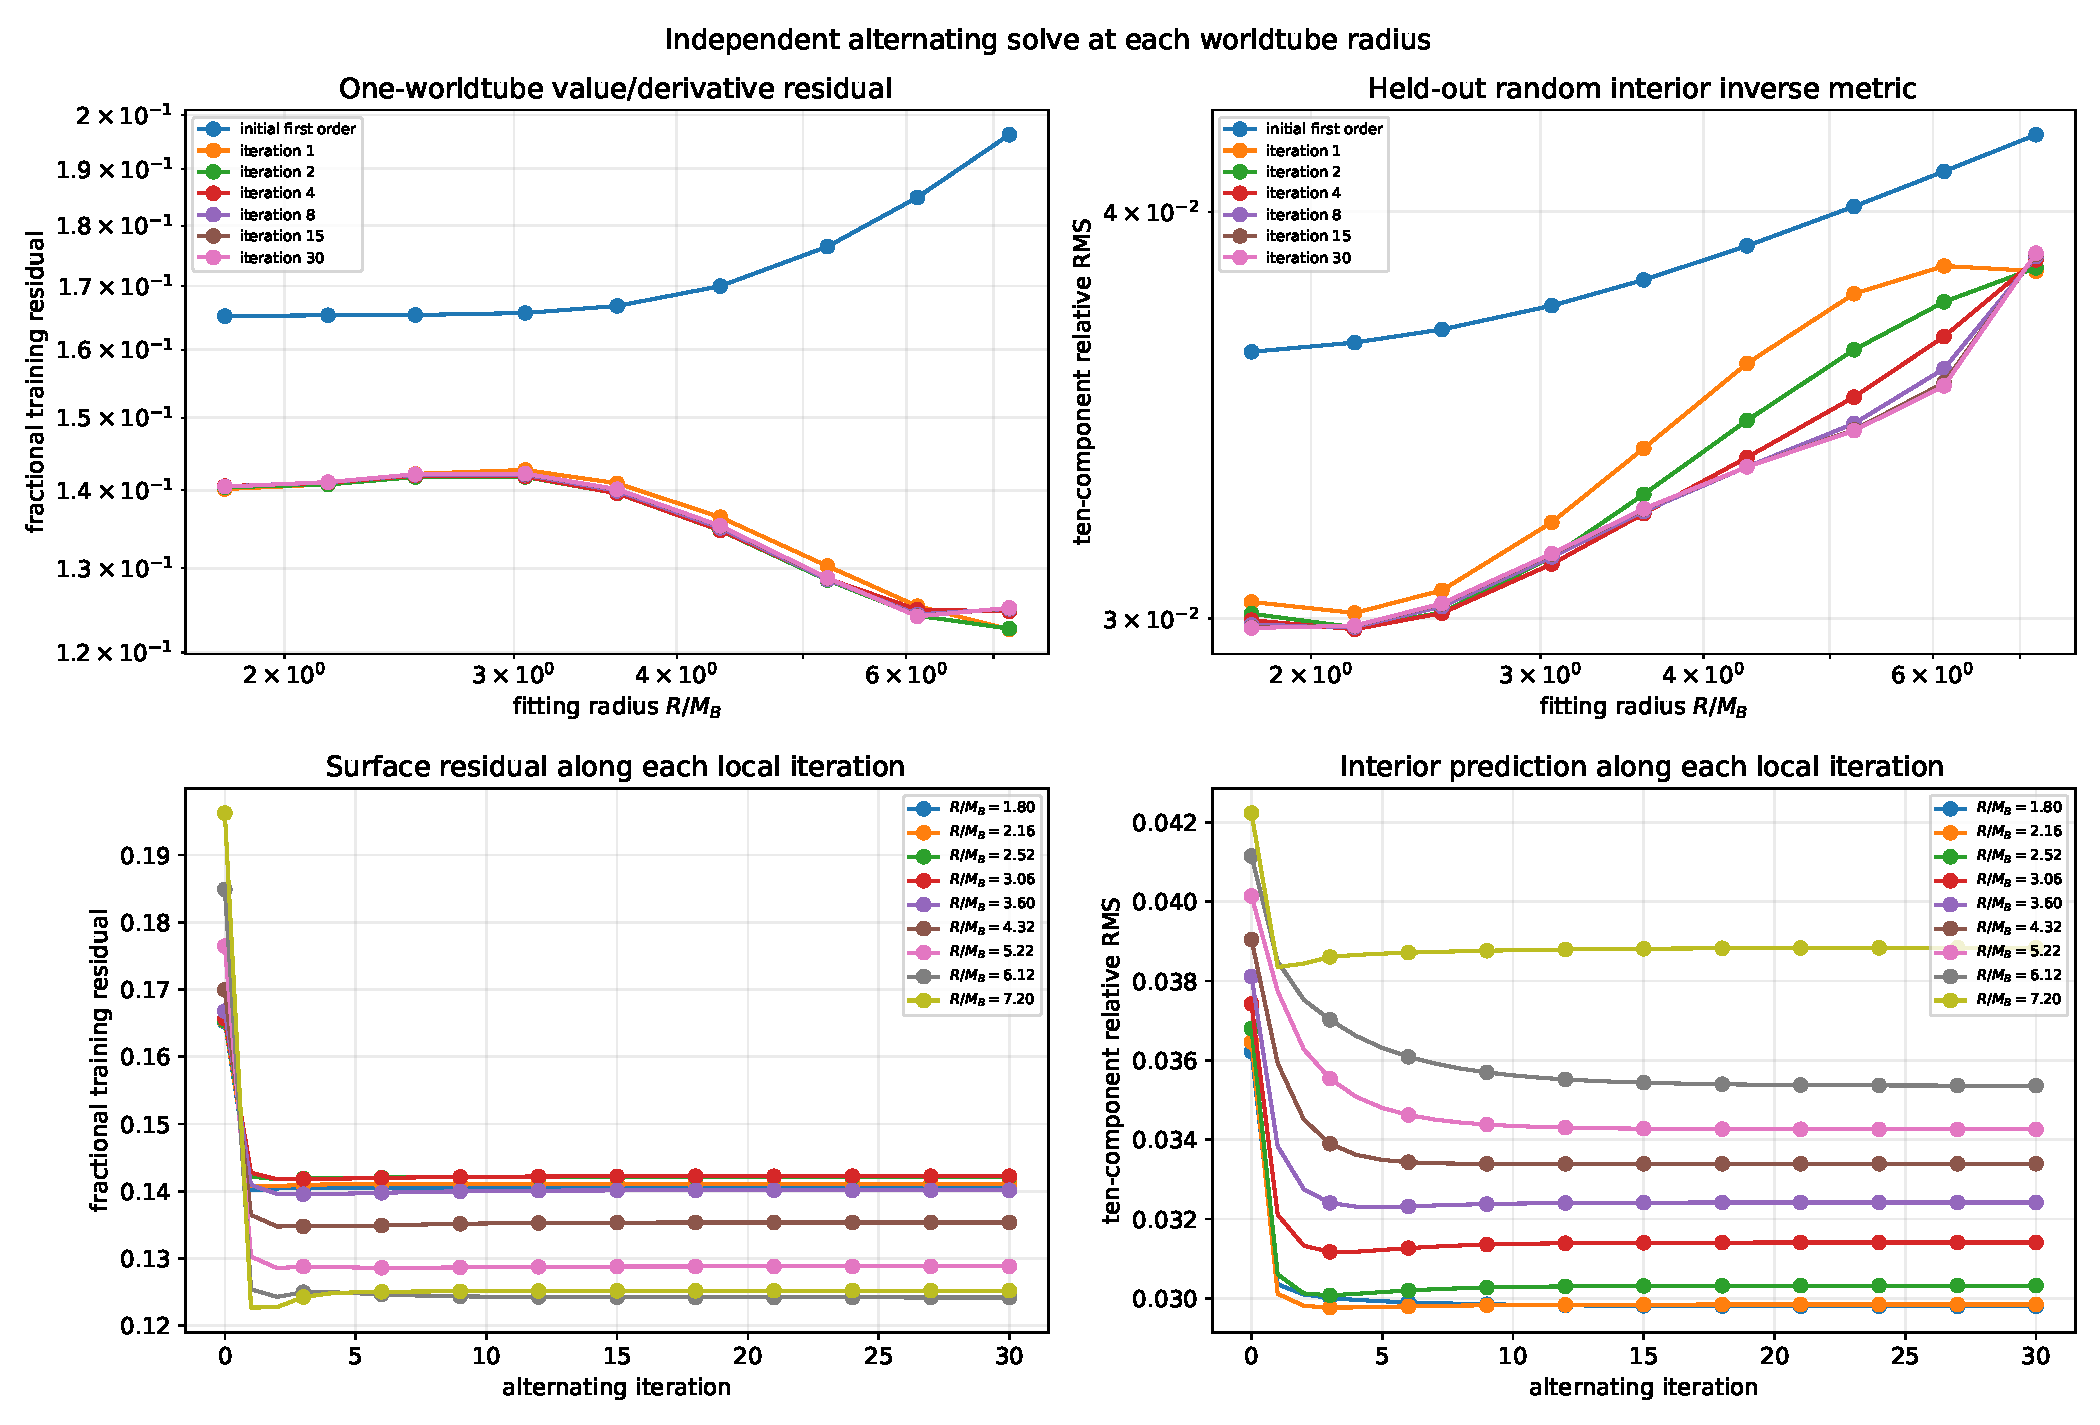
\includegraphics[width=0.96\textwidth]{q8_t950_radius_by_radius_iteration.pdf}
\caption{Radius-by-radius Gauss--Seidel iteration.  Surface and interior
diagnostics generally prefer different stopping times.}
\label{fig:iteration}
\end{figure}

\section{Time derivatives and evolution consistency}

The first-order generalized-harmonic variables provide
\begin{equation}
\partial_Tg_{ab}
=\beta^i\Phi_{iab}-\alpha\Pi_{ab},
\qquad
\partial_T\G^{ab}
=-\G^{ac}\G^{bd}\partial_Tg_{cd}.
\end{equation}
At fixed local coordinates on a sphere moving with velocity
\(v_{\rm center}^i\),
\begin{equation}
D_T\G^{ab}
=\partial_T\G^{ab}
+v_{\rm center}^i\partial_i\G^{ab}.
\label{eq:comoving-derivative}
\end{equation}
The \(\Pi,\Phi\)-constructed derivative agrees with a time derivative of
independently interpolated moving-sphere data to approximately
\(2\times10^{-4}\) at \(R=0.2M_{\rm tot}\).

Let
\begin{equation}
a=\dot q^0,
\qquad
\Lambda_{ij}=L_{ij}/M_B.
\end{equation}
Since \(T=t+q^0(t)\),
\begin{equation}
\ddot q^0=(1+a)\frac{da}{dT},
\qquad
\dot L_{ij}=M_B(1+a)\frac{d\Lambda_{ij}}{dT}.
\end{equation}
At \(R=0.2M_{\rm tot}\), the directly measured scales are
\begin{center}
\begin{tabular}{lccc}
\toprule
 & \(\Pi,\Phi\) direct & finite difference & free second-order fit\\
\midrule
\(\operatorname{RMS}|\ddot q^0|\) &
\(3.95\times10^{-5}\) & \(4.42\times10^{-5}\) &
\(4.08\times10^{-2}\)\\
\(\operatorname{RMS}|M_B\dot\Lambda|\) &
\(1.25\times10^{-5}\) & \(1.96\times10^{-5}\) &
\(7.16\times10^{-3}\)\\
\bottomrule
\end{tabular}
\end{center}

The freely fitted time jets are therefore inflated by roughly three orders
of magnitude.  They act as effective residual-reduction directions rather
than physical derivatives.  Moreover, the true vector rates
\(\dot b_i\) and \(\ddot q^i\) have norms of a few \(10^{-3}\), larger than
the physical clock and strain rates.  They cannot be omitted from a
dynamical second-order subsystem.

\begin{figure}[htbp]
\centering
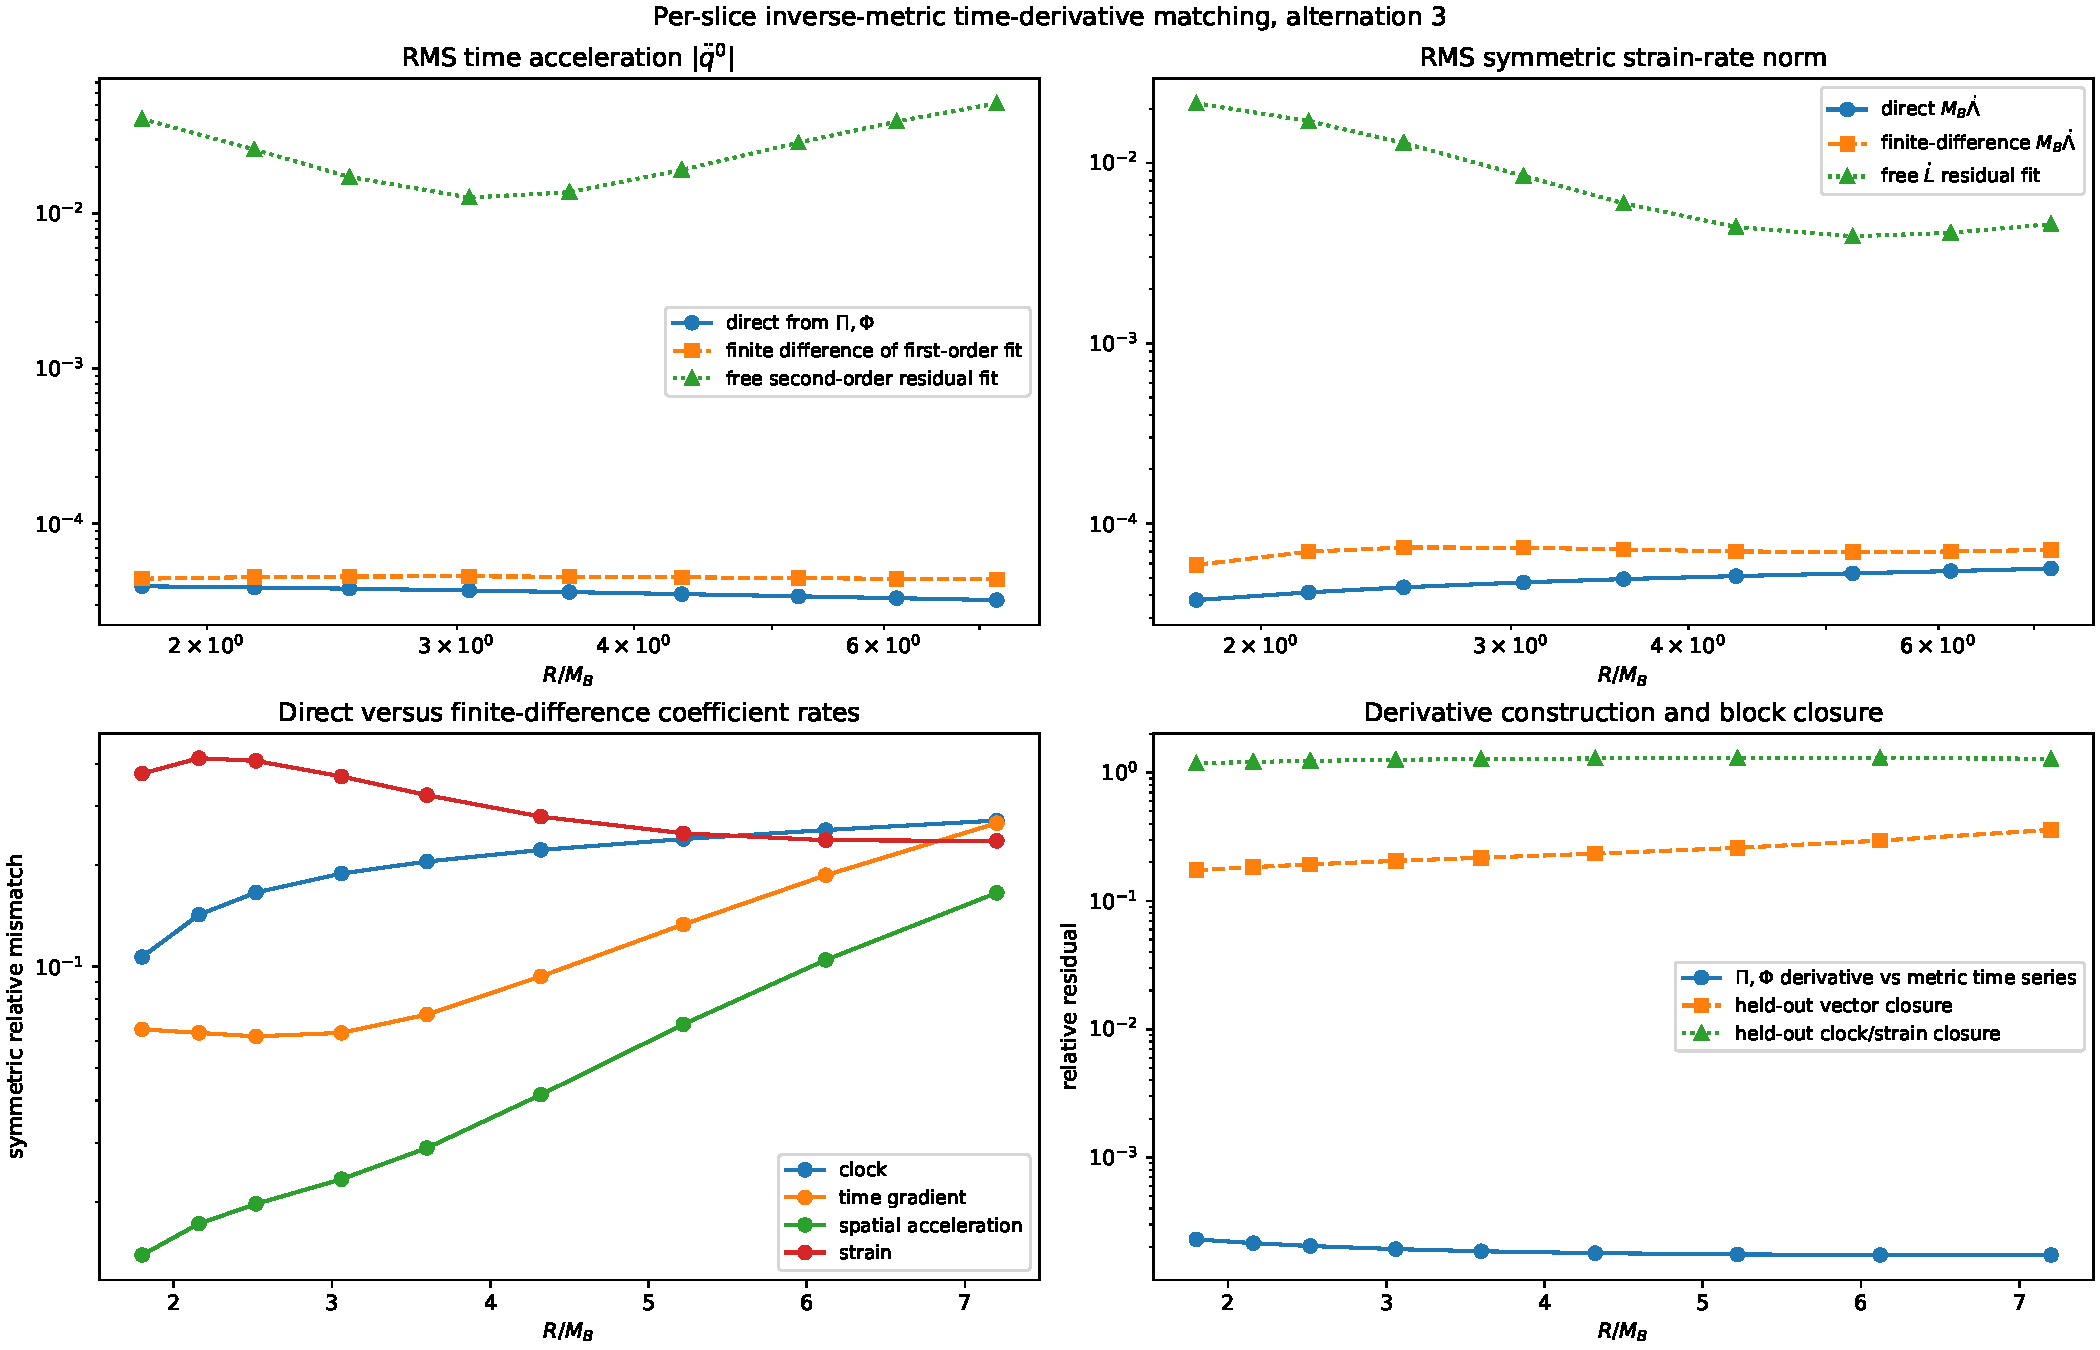
\includegraphics[width=0.96\textwidth]{q8_direct_metric_time_derivative.pdf}
\caption{Direct \(\Pi,\Phi\) measurements, finite differences of the
first-order history, and freely fitted second-order rates.}
\label{fig:time-derivative}
\end{figure}

\subsection{First-order evolution and center velocity}

Integrating the direct rates from one initial value reproduces the evolution
of \(\dot q^i\) to \(1.36\%\) and that of \(\dot q^0\) to \(10.4\%\) at the
smallest radius.

The curvature-center velocity gives the absolute kinematic relation
\begin{equation}
\dot q^i
=(1+\dot q^0)\frac{dz_{\rm center}^i}{dT}.
\end{equation}
It agrees with the algebraic metric fit to \(2.3\%\) at \(R=0.2M_{\rm tot}\)
and approximately \(2.1\%\) at \(R=0.28M_{\rm tot}\).  Omitting the
time-coordinate factor gives an error near \(10\%\).

\begin{figure}[htbp]
\centering
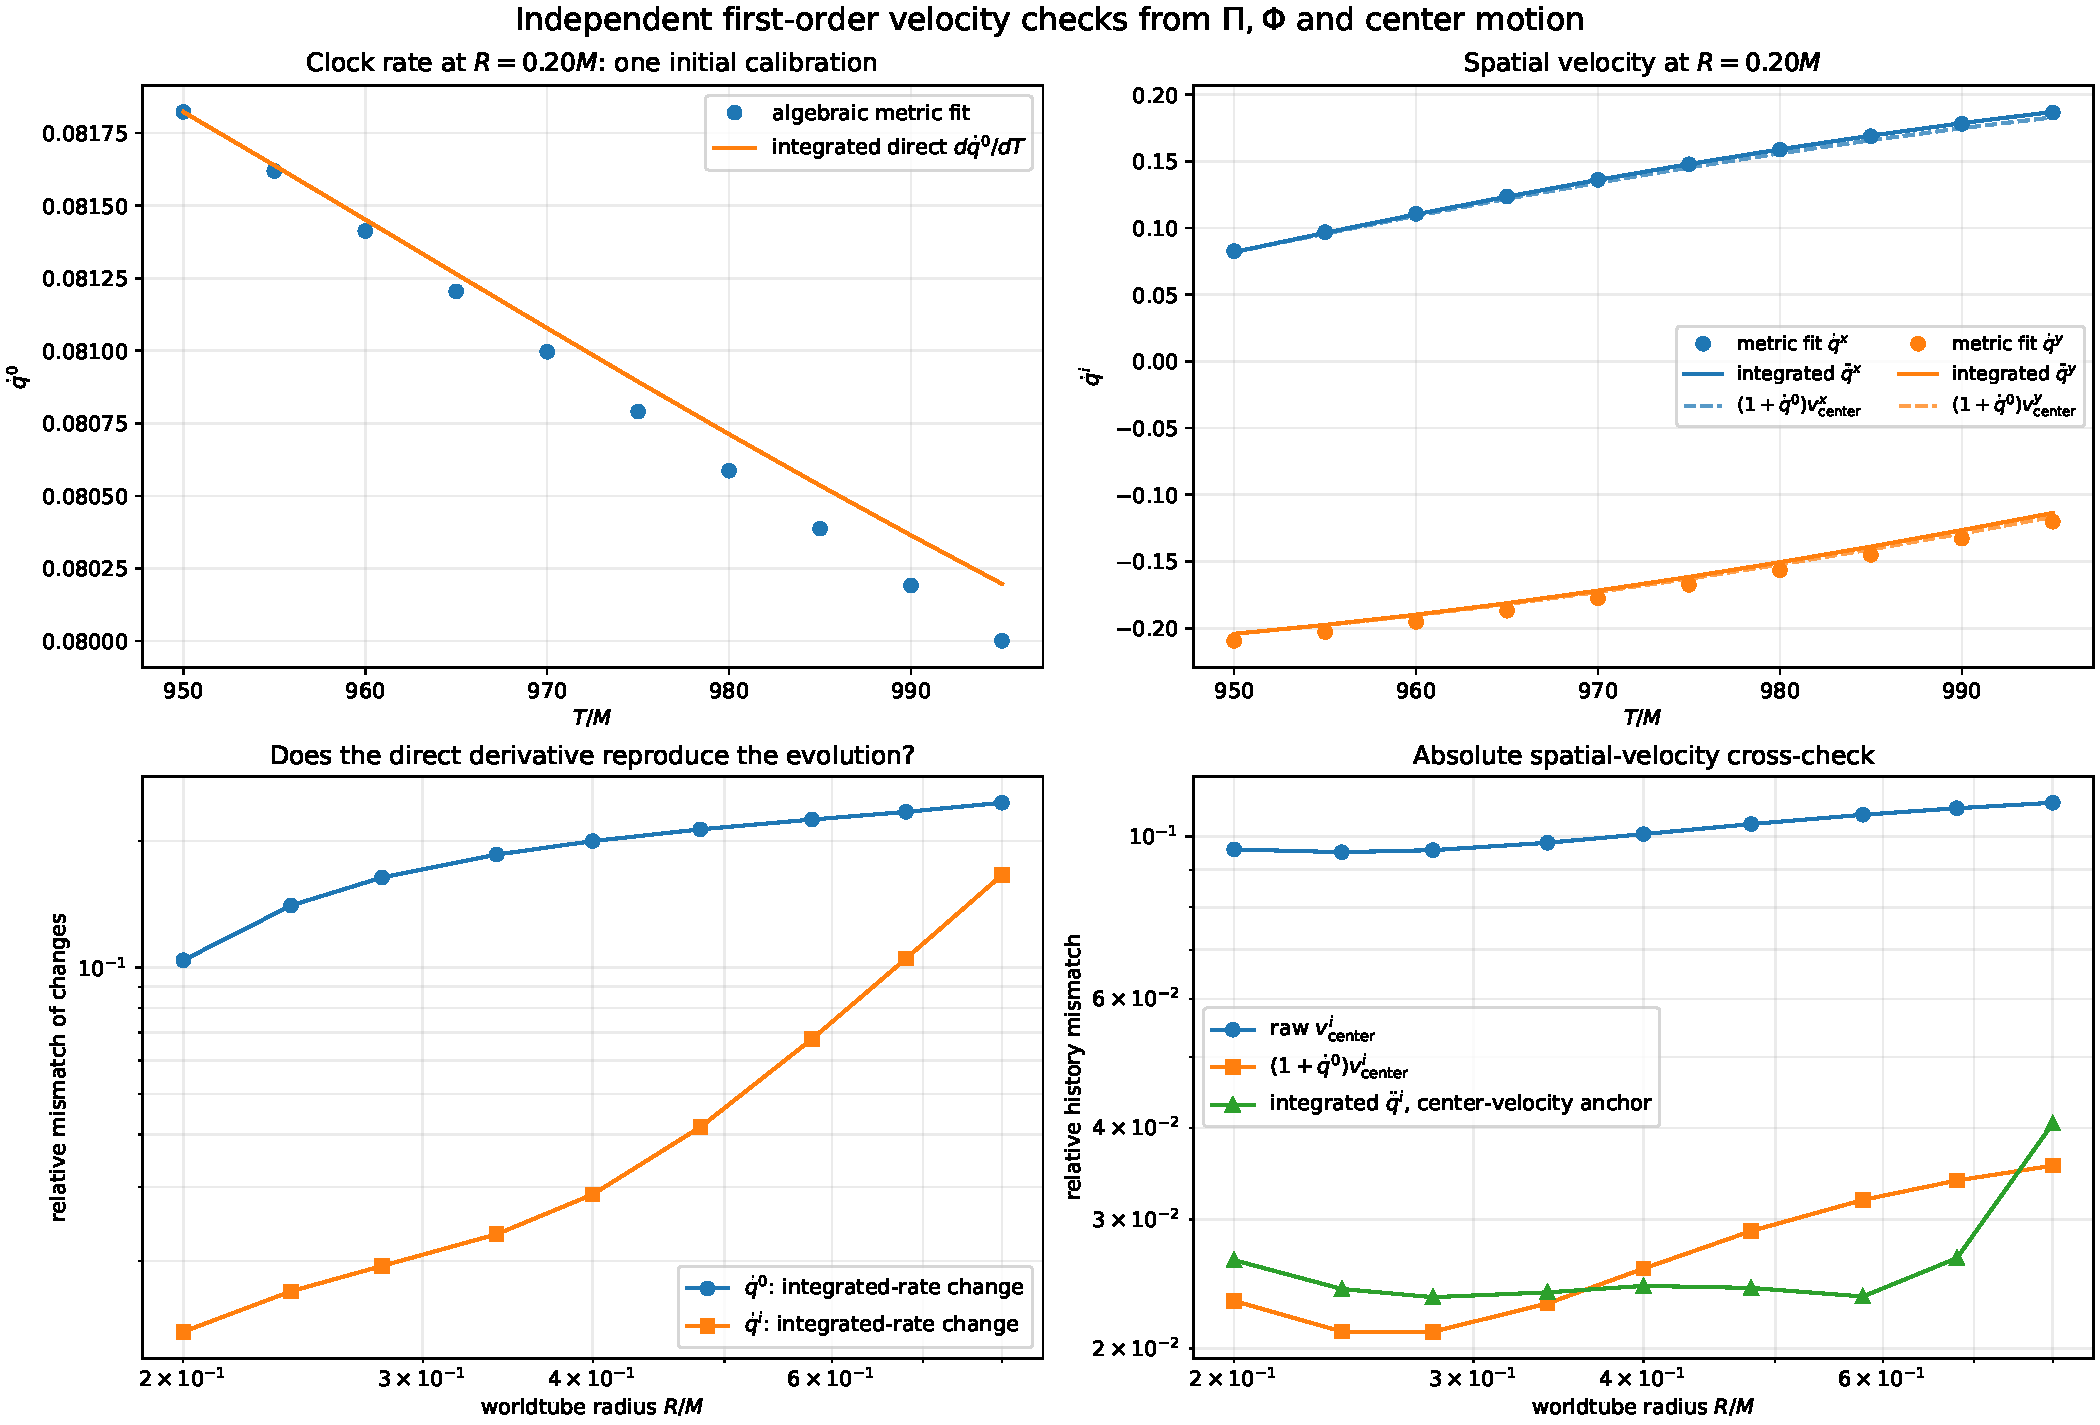
\includegraphics[width=0.96\textwidth]{q8_first_order_kinematic_reconstruction.pdf}
\caption{Independent first-order velocity checks from direct metric
derivatives and curvature-center motion.}
\label{fig:kinematic}
\end{figure}

\subsection{Metric-only translation velocity}

The comoving derivative in \cref{eq:comoving-derivative} cancels center
translation and measures \(\ddot q^i\).  The fixed-inertial derivative instead
satisfies
\begin{equation}
\partial_T\G^{ab}
=-\partial_i\G_{(0)}^{ab}\frac{dq^i}{dT}
+\sum_A\Rop_A^{ab}\frac{dp_A}{dT}.
\end{equation}
A preliminary full-rank sixteen-parameter fit gives a metric-only center
velocity.  At \(R=0.2M_{\rm tot}\), it agrees with the Kretschmann-center
velocity to approximately \(2.7\%\), and the corresponding harmonic-time
\(\dot q^i\) agrees with the algebraic first-order fit to approximately
\(4.9\%\).

There is no analogous absolute \(q^0\) translation measurement because the
Schwarzschild background is stationary.  The derivative determines
\(\ddot q^0\); \(\dot q^0\) still requires an algebraic fit or one initial
calibration.

\section{Limitations}

\begin{itemize}
  \item The q4 \(T=850M_{\rm tot}\) production slice has no matched
        fine-resolution copy; the downloaded fine data stop near
        \(T=700M_{\rm tot}\).
  \item The q8 study uses full-resolution output, but \(q=8\) is not yet an
        asymptotically small mass ratio.
  \item The q4 small black hole had a residual spin dominated by
        \(\chi_z\simeq-2.23\times10^{-4}\).  Spin has not been added to the
        background model.
  \item The multi-slice analysis spans \(45M_{\rm tot}\).  Direct per-slice
        derivatives remove the main cadence limitation, but longer histories
        are needed for dynamical stability tests.
  \item The magnetic response remains the least well verified analytic and
        numerical sector.
  \item A small training residual is never sufficient evidence of physical
        parameter recovery.
\end{itemize}

\section{Current assessment}

The analysis supports the following picture:

\begin{enumerate}
  \item The corrected coordinate-map and response algebra is internally
        consistent for the implemented families.
  \item First order gives a large and robust improvement over centered
        Schwarzschild.
  \item V1 is the strongest current vector estimator, and radial derivatives
        modestly improve it.
  \item C3 is the most conservative current clock/strain estimator, although
        its closure remains weaker.
  \item The complete triangular second-order solve is not physically
        validated despite passing every manufactured algebraic test.
  \item Useful second-order information is concentrated in spatial-strain
        rate, time acceleration, and the polar-\(J=2\) response space.
  \item Radial derivatives add genuine information at both first and second
        order.
  \item Direct time derivatives must replace or constrain freely fitted
        evolution jets.
  \item A few Gauss--Seidel sweeps can decontaminate the two orders, but the
        iteration requires validation-based early stopping.
  \item The fixed-inertial metric derivative supplies an independent
        measurement of spatial center velocity.
\end{enumerate}

The emerging construction is therefore a hierarchy of physically organized
overdetermined systems rather than one unrestricted global least-squares fit.
Each block must be judged by radius stability, omitted-block closure,
derivative consistency, and held-out interior prediction.

\appendix
\section{Compact numerical summary}

\begin{center}
\small
\begin{tabularx}{0.98\textwidth}{
  >{\raggedright\arraybackslash}p{0.31\textwidth}
  >{\raggedright\arraybackslash}p{0.22\textwidth}X}
\toprule
\textbf{test} & \textbf{representative value} & \textbf{interpretation}\\
\midrule
q8 Schwarzschild interior error & \(2.21\times10^{-1}\) &
zeroth-order baseline\\
q8 V1+C3 interior error & \(3.61\times10^{-2}\) &
factor \(6.14\) improvement\\
derivative-assisted first order & \(3.57\times10^{-2}\) &
small vector-sector improvement\\
seven-parameter second order with radial derivative &
\(3.17\)--\(3.19\times10^{-2}\) &
conservative useful second-order block\\
polar-\(J=2\) targeted fit & \(3.13\times10^{-2}\) &
strongest targeted 15-parameter subsystem\\
globally balanced 43-column fit & \(3.01\times10^{-2}\) &
useful aggregate response, not individual identification\\
radius-by-radius alternation at \(R=0.24M\) &
\(2.98\times10^{-2}\) after 3 sweeps &
supports early-stopped decontamination\\
direct clock acceleration & \(3.95\times10^{-5}\) &
free fit overestimates by about \(10^3\)\\
direct spatial velocity evolution & \(1.36\%\) mismatch &
strong dynamical consistency\\
metric-only center velocity & \(2.7\%\) mismatch &
preliminary fixed-inertial derivative result\\
\bottomrule
\end{tabularx}
\end{center}

\section{Companion artifacts}

\begin{itemize}
  \item \texttt{q8\_first\_order\_matching.ipynb}: complete executed
        single-slice analysis.
  \item \texttt{build\_q8\_first\_order\_notebook.py}: reproducible notebook
        source.
  \item \texttt{temporal\_ode\_consistency/}: ten-slice and direct
        \(\Pi,\Phi\) derivative analyses.
  \item \texttt{gauge-matching-audit/}: analytic audit, Mathematica notebooks,
        focused q4 notebooks, and provenance.
\end{itemize}

\end{document}
